
% Default to the notebook output style

    


% Inherit from the specified cell style.




    
\documentclass[11pt]{article}

    
    
    \usepackage[T1]{fontenc}
    % Nicer default font (+ math font) than Computer Modern for most use cases
    \usepackage{mathpazo}

    % Basic figure setup, for now with no caption control since it's done
    % automatically by Pandoc (which extracts ![](path) syntax from Markdown).
    \usepackage{graphicx}
    % We will generate all images so they have a width \maxwidth. This means
    % that they will get their normal width if they fit onto the page, but
    % are scaled down if they would overflow the margins.
    \makeatletter
    \def\maxwidth{\ifdim\Gin@nat@width>\linewidth\linewidth
    \else\Gin@nat@width\fi}
    \makeatother
    \let\Oldincludegraphics\includegraphics
    % Set max figure width to be 80% of text width, for now hardcoded.
    \renewcommand{\includegraphics}[1]{\Oldincludegraphics[width=.8\maxwidth]{#1}}
    % Ensure that by default, figures have no caption (until we provide a
    % proper Figure object with a Caption API and a way to capture that
    % in the conversion process - todo).
    \usepackage{caption}
    \DeclareCaptionLabelFormat{nolabel}{}
    \captionsetup{labelformat=nolabel}

    \usepackage{adjustbox} % Used to constrain images to a maximum size 
    \usepackage{xcolor} % Allow colors to be defined
    \usepackage{enumerate} % Needed for markdown enumerations to work
    \usepackage{geometry} % Used to adjust the document margins
    \usepackage{amsmath} % Equations
    \usepackage{amssymb} % Equations
    \usepackage{textcomp} % defines textquotesingle
    % Hack from http://tex.stackexchange.com/a/47451/13684:
    \AtBeginDocument{%
        \def\PYZsq{\textquotesingle}% Upright quotes in Pygmentized code
    }
    \usepackage{upquote} % Upright quotes for verbatim code
    \usepackage{eurosym} % defines \euro
    \usepackage[mathletters]{ucs} % Extended unicode (utf-8) support
    \usepackage[utf8x]{inputenc} % Allow utf-8 characters in the tex document
    \usepackage{fancyvrb} % verbatim replacement that allows latex
    \usepackage{grffile} % extends the file name processing of package graphics 
                         % to support a larger range 
    % The hyperref package gives us a pdf with properly built
    % internal navigation ('pdf bookmarks' for the table of contents,
    % internal cross-reference links, web links for URLs, etc.)
    \usepackage{hyperref}
    \usepackage{longtable} % longtable support required by pandoc >1.10
    \usepackage{booktabs}  % table support for pandoc > 1.12.2
    \usepackage[inline]{enumitem} % IRkernel/repr support (it uses the enumerate* environment)
    \usepackage[normalem]{ulem} % ulem is needed to support strikethroughs (\sout)
                                % normalem makes italics be italics, not underlines
    

    
    
    % Colors for the hyperref package
    \definecolor{urlcolor}{rgb}{0,.145,.698}
    \definecolor{linkcolor}{rgb}{.71,0.21,0.01}
    \definecolor{citecolor}{rgb}{.12,.54,.11}

    % ANSI colors
    \definecolor{ansi-black}{HTML}{3E424D}
    \definecolor{ansi-black-intense}{HTML}{282C36}
    \definecolor{ansi-red}{HTML}{E75C58}
    \definecolor{ansi-red-intense}{HTML}{B22B31}
    \definecolor{ansi-green}{HTML}{00A250}
    \definecolor{ansi-green-intense}{HTML}{007427}
    \definecolor{ansi-yellow}{HTML}{DDB62B}
    \definecolor{ansi-yellow-intense}{HTML}{B27D12}
    \definecolor{ansi-blue}{HTML}{208FFB}
    \definecolor{ansi-blue-intense}{HTML}{0065CA}
    \definecolor{ansi-magenta}{HTML}{D160C4}
    \definecolor{ansi-magenta-intense}{HTML}{A03196}
    \definecolor{ansi-cyan}{HTML}{60C6C8}
    \definecolor{ansi-cyan-intense}{HTML}{258F8F}
    \definecolor{ansi-white}{HTML}{C5C1B4}
    \definecolor{ansi-white-intense}{HTML}{A1A6B2}

    % commands and environments needed by pandoc snippets
    % extracted from the output of `pandoc -s`
    \providecommand{\tightlist}{%
      \setlength{\itemsep}{0pt}\setlength{\parskip}{0pt}}
    \DefineVerbatimEnvironment{Highlighting}{Verbatim}{commandchars=\\\{\}}
    % Add ',fontsize=\small' for more characters per line
    \newenvironment{Shaded}{}{}
    \newcommand{\KeywordTok}[1]{\textcolor[rgb]{0.00,0.44,0.13}{\textbf{{#1}}}}
    \newcommand{\DataTypeTok}[1]{\textcolor[rgb]{0.56,0.13,0.00}{{#1}}}
    \newcommand{\DecValTok}[1]{\textcolor[rgb]{0.25,0.63,0.44}{{#1}}}
    \newcommand{\BaseNTok}[1]{\textcolor[rgb]{0.25,0.63,0.44}{{#1}}}
    \newcommand{\FloatTok}[1]{\textcolor[rgb]{0.25,0.63,0.44}{{#1}}}
    \newcommand{\CharTok}[1]{\textcolor[rgb]{0.25,0.44,0.63}{{#1}}}
    \newcommand{\StringTok}[1]{\textcolor[rgb]{0.25,0.44,0.63}{{#1}}}
    \newcommand{\CommentTok}[1]{\textcolor[rgb]{0.38,0.63,0.69}{\textit{{#1}}}}
    \newcommand{\OtherTok}[1]{\textcolor[rgb]{0.00,0.44,0.13}{{#1}}}
    \newcommand{\AlertTok}[1]{\textcolor[rgb]{1.00,0.00,0.00}{\textbf{{#1}}}}
    \newcommand{\FunctionTok}[1]{\textcolor[rgb]{0.02,0.16,0.49}{{#1}}}
    \newcommand{\RegionMarkerTok}[1]{{#1}}
    \newcommand{\ErrorTok}[1]{\textcolor[rgb]{1.00,0.00,0.00}{\textbf{{#1}}}}
    \newcommand{\NormalTok}[1]{{#1}}
    
    % Additional commands for more recent versions of Pandoc
    \newcommand{\ConstantTok}[1]{\textcolor[rgb]{0.53,0.00,0.00}{{#1}}}
    \newcommand{\SpecialCharTok}[1]{\textcolor[rgb]{0.25,0.44,0.63}{{#1}}}
    \newcommand{\VerbatimStringTok}[1]{\textcolor[rgb]{0.25,0.44,0.63}{{#1}}}
    \newcommand{\SpecialStringTok}[1]{\textcolor[rgb]{0.73,0.40,0.53}{{#1}}}
    \newcommand{\ImportTok}[1]{{#1}}
    \newcommand{\DocumentationTok}[1]{\textcolor[rgb]{0.73,0.13,0.13}{\textit{{#1}}}}
    \newcommand{\AnnotationTok}[1]{\textcolor[rgb]{0.38,0.63,0.69}{\textbf{\textit{{#1}}}}}
    \newcommand{\CommentVarTok}[1]{\textcolor[rgb]{0.38,0.63,0.69}{\textbf{\textit{{#1}}}}}
    \newcommand{\VariableTok}[1]{\textcolor[rgb]{0.10,0.09,0.49}{{#1}}}
    \newcommand{\ControlFlowTok}[1]{\textcolor[rgb]{0.00,0.44,0.13}{\textbf{{#1}}}}
    \newcommand{\OperatorTok}[1]{\textcolor[rgb]{0.40,0.40,0.40}{{#1}}}
    \newcommand{\BuiltInTok}[1]{{#1}}
    \newcommand{\ExtensionTok}[1]{{#1}}
    \newcommand{\PreprocessorTok}[1]{\textcolor[rgb]{0.74,0.48,0.00}{{#1}}}
    \newcommand{\AttributeTok}[1]{\textcolor[rgb]{0.49,0.56,0.16}{{#1}}}
    \newcommand{\InformationTok}[1]{\textcolor[rgb]{0.38,0.63,0.69}{\textbf{\textit{{#1}}}}}
    \newcommand{\WarningTok}[1]{\textcolor[rgb]{0.38,0.63,0.69}{\textbf{\textit{{#1}}}}}
    
    
    % Define a nice break command that doesn't care if a line doesn't already
    % exist.
    \def\br{\hspace*{\fill} \\* }
    % Math Jax compatability definitions
    \def\gt{>}
    \def\lt{<}
    % Document parameters
    \title{DIP-HW13}
    
    
    

    % Pygments definitions
    
\makeatletter
\def\PY@reset{\let\PY@it=\relax \let\PY@bf=\relax%
    \let\PY@ul=\relax \let\PY@tc=\relax%
    \let\PY@bc=\relax \let\PY@ff=\relax}
\def\PY@tok#1{\csname PY@tok@#1\endcsname}
\def\PY@toks#1+{\ifx\relax#1\empty\else%
    \PY@tok{#1}\expandafter\PY@toks\fi}
\def\PY@do#1{\PY@bc{\PY@tc{\PY@ul{%
    \PY@it{\PY@bf{\PY@ff{#1}}}}}}}
\def\PY#1#2{\PY@reset\PY@toks#1+\relax+\PY@do{#2}}

\expandafter\def\csname PY@tok@w\endcsname{\def\PY@tc##1{\textcolor[rgb]{0.73,0.73,0.73}{##1}}}
\expandafter\def\csname PY@tok@c\endcsname{\let\PY@it=\textit\def\PY@tc##1{\textcolor[rgb]{0.25,0.50,0.50}{##1}}}
\expandafter\def\csname PY@tok@cp\endcsname{\def\PY@tc##1{\textcolor[rgb]{0.74,0.48,0.00}{##1}}}
\expandafter\def\csname PY@tok@k\endcsname{\let\PY@bf=\textbf\def\PY@tc##1{\textcolor[rgb]{0.00,0.50,0.00}{##1}}}
\expandafter\def\csname PY@tok@kp\endcsname{\def\PY@tc##1{\textcolor[rgb]{0.00,0.50,0.00}{##1}}}
\expandafter\def\csname PY@tok@kt\endcsname{\def\PY@tc##1{\textcolor[rgb]{0.69,0.00,0.25}{##1}}}
\expandafter\def\csname PY@tok@o\endcsname{\def\PY@tc##1{\textcolor[rgb]{0.40,0.40,0.40}{##1}}}
\expandafter\def\csname PY@tok@ow\endcsname{\let\PY@bf=\textbf\def\PY@tc##1{\textcolor[rgb]{0.67,0.13,1.00}{##1}}}
\expandafter\def\csname PY@tok@nb\endcsname{\def\PY@tc##1{\textcolor[rgb]{0.00,0.50,0.00}{##1}}}
\expandafter\def\csname PY@tok@nf\endcsname{\def\PY@tc##1{\textcolor[rgb]{0.00,0.00,1.00}{##1}}}
\expandafter\def\csname PY@tok@nc\endcsname{\let\PY@bf=\textbf\def\PY@tc##1{\textcolor[rgb]{0.00,0.00,1.00}{##1}}}
\expandafter\def\csname PY@tok@nn\endcsname{\let\PY@bf=\textbf\def\PY@tc##1{\textcolor[rgb]{0.00,0.00,1.00}{##1}}}
\expandafter\def\csname PY@tok@ne\endcsname{\let\PY@bf=\textbf\def\PY@tc##1{\textcolor[rgb]{0.82,0.25,0.23}{##1}}}
\expandafter\def\csname PY@tok@nv\endcsname{\def\PY@tc##1{\textcolor[rgb]{0.10,0.09,0.49}{##1}}}
\expandafter\def\csname PY@tok@no\endcsname{\def\PY@tc##1{\textcolor[rgb]{0.53,0.00,0.00}{##1}}}
\expandafter\def\csname PY@tok@nl\endcsname{\def\PY@tc##1{\textcolor[rgb]{0.63,0.63,0.00}{##1}}}
\expandafter\def\csname PY@tok@ni\endcsname{\let\PY@bf=\textbf\def\PY@tc##1{\textcolor[rgb]{0.60,0.60,0.60}{##1}}}
\expandafter\def\csname PY@tok@na\endcsname{\def\PY@tc##1{\textcolor[rgb]{0.49,0.56,0.16}{##1}}}
\expandafter\def\csname PY@tok@nt\endcsname{\let\PY@bf=\textbf\def\PY@tc##1{\textcolor[rgb]{0.00,0.50,0.00}{##1}}}
\expandafter\def\csname PY@tok@nd\endcsname{\def\PY@tc##1{\textcolor[rgb]{0.67,0.13,1.00}{##1}}}
\expandafter\def\csname PY@tok@s\endcsname{\def\PY@tc##1{\textcolor[rgb]{0.73,0.13,0.13}{##1}}}
\expandafter\def\csname PY@tok@sd\endcsname{\let\PY@it=\textit\def\PY@tc##1{\textcolor[rgb]{0.73,0.13,0.13}{##1}}}
\expandafter\def\csname PY@tok@si\endcsname{\let\PY@bf=\textbf\def\PY@tc##1{\textcolor[rgb]{0.73,0.40,0.53}{##1}}}
\expandafter\def\csname PY@tok@se\endcsname{\let\PY@bf=\textbf\def\PY@tc##1{\textcolor[rgb]{0.73,0.40,0.13}{##1}}}
\expandafter\def\csname PY@tok@sr\endcsname{\def\PY@tc##1{\textcolor[rgb]{0.73,0.40,0.53}{##1}}}
\expandafter\def\csname PY@tok@ss\endcsname{\def\PY@tc##1{\textcolor[rgb]{0.10,0.09,0.49}{##1}}}
\expandafter\def\csname PY@tok@sx\endcsname{\def\PY@tc##1{\textcolor[rgb]{0.00,0.50,0.00}{##1}}}
\expandafter\def\csname PY@tok@m\endcsname{\def\PY@tc##1{\textcolor[rgb]{0.40,0.40,0.40}{##1}}}
\expandafter\def\csname PY@tok@gh\endcsname{\let\PY@bf=\textbf\def\PY@tc##1{\textcolor[rgb]{0.00,0.00,0.50}{##1}}}
\expandafter\def\csname PY@tok@gu\endcsname{\let\PY@bf=\textbf\def\PY@tc##1{\textcolor[rgb]{0.50,0.00,0.50}{##1}}}
\expandafter\def\csname PY@tok@gd\endcsname{\def\PY@tc##1{\textcolor[rgb]{0.63,0.00,0.00}{##1}}}
\expandafter\def\csname PY@tok@gi\endcsname{\def\PY@tc##1{\textcolor[rgb]{0.00,0.63,0.00}{##1}}}
\expandafter\def\csname PY@tok@gr\endcsname{\def\PY@tc##1{\textcolor[rgb]{1.00,0.00,0.00}{##1}}}
\expandafter\def\csname PY@tok@ge\endcsname{\let\PY@it=\textit}
\expandafter\def\csname PY@tok@gs\endcsname{\let\PY@bf=\textbf}
\expandafter\def\csname PY@tok@gp\endcsname{\let\PY@bf=\textbf\def\PY@tc##1{\textcolor[rgb]{0.00,0.00,0.50}{##1}}}
\expandafter\def\csname PY@tok@go\endcsname{\def\PY@tc##1{\textcolor[rgb]{0.53,0.53,0.53}{##1}}}
\expandafter\def\csname PY@tok@gt\endcsname{\def\PY@tc##1{\textcolor[rgb]{0.00,0.27,0.87}{##1}}}
\expandafter\def\csname PY@tok@err\endcsname{\def\PY@bc##1{\setlength{\fboxsep}{0pt}\fcolorbox[rgb]{1.00,0.00,0.00}{1,1,1}{\strut ##1}}}
\expandafter\def\csname PY@tok@kc\endcsname{\let\PY@bf=\textbf\def\PY@tc##1{\textcolor[rgb]{0.00,0.50,0.00}{##1}}}
\expandafter\def\csname PY@tok@kd\endcsname{\let\PY@bf=\textbf\def\PY@tc##1{\textcolor[rgb]{0.00,0.50,0.00}{##1}}}
\expandafter\def\csname PY@tok@kn\endcsname{\let\PY@bf=\textbf\def\PY@tc##1{\textcolor[rgb]{0.00,0.50,0.00}{##1}}}
\expandafter\def\csname PY@tok@kr\endcsname{\let\PY@bf=\textbf\def\PY@tc##1{\textcolor[rgb]{0.00,0.50,0.00}{##1}}}
\expandafter\def\csname PY@tok@bp\endcsname{\def\PY@tc##1{\textcolor[rgb]{0.00,0.50,0.00}{##1}}}
\expandafter\def\csname PY@tok@fm\endcsname{\def\PY@tc##1{\textcolor[rgb]{0.00,0.00,1.00}{##1}}}
\expandafter\def\csname PY@tok@vc\endcsname{\def\PY@tc##1{\textcolor[rgb]{0.10,0.09,0.49}{##1}}}
\expandafter\def\csname PY@tok@vg\endcsname{\def\PY@tc##1{\textcolor[rgb]{0.10,0.09,0.49}{##1}}}
\expandafter\def\csname PY@tok@vi\endcsname{\def\PY@tc##1{\textcolor[rgb]{0.10,0.09,0.49}{##1}}}
\expandafter\def\csname PY@tok@vm\endcsname{\def\PY@tc##1{\textcolor[rgb]{0.10,0.09,0.49}{##1}}}
\expandafter\def\csname PY@tok@sa\endcsname{\def\PY@tc##1{\textcolor[rgb]{0.73,0.13,0.13}{##1}}}
\expandafter\def\csname PY@tok@sb\endcsname{\def\PY@tc##1{\textcolor[rgb]{0.73,0.13,0.13}{##1}}}
\expandafter\def\csname PY@tok@sc\endcsname{\def\PY@tc##1{\textcolor[rgb]{0.73,0.13,0.13}{##1}}}
\expandafter\def\csname PY@tok@dl\endcsname{\def\PY@tc##1{\textcolor[rgb]{0.73,0.13,0.13}{##1}}}
\expandafter\def\csname PY@tok@s2\endcsname{\def\PY@tc##1{\textcolor[rgb]{0.73,0.13,0.13}{##1}}}
\expandafter\def\csname PY@tok@sh\endcsname{\def\PY@tc##1{\textcolor[rgb]{0.73,0.13,0.13}{##1}}}
\expandafter\def\csname PY@tok@s1\endcsname{\def\PY@tc##1{\textcolor[rgb]{0.73,0.13,0.13}{##1}}}
\expandafter\def\csname PY@tok@mb\endcsname{\def\PY@tc##1{\textcolor[rgb]{0.40,0.40,0.40}{##1}}}
\expandafter\def\csname PY@tok@mf\endcsname{\def\PY@tc##1{\textcolor[rgb]{0.40,0.40,0.40}{##1}}}
\expandafter\def\csname PY@tok@mh\endcsname{\def\PY@tc##1{\textcolor[rgb]{0.40,0.40,0.40}{##1}}}
\expandafter\def\csname PY@tok@mi\endcsname{\def\PY@tc##1{\textcolor[rgb]{0.40,0.40,0.40}{##1}}}
\expandafter\def\csname PY@tok@il\endcsname{\def\PY@tc##1{\textcolor[rgb]{0.40,0.40,0.40}{##1}}}
\expandafter\def\csname PY@tok@mo\endcsname{\def\PY@tc##1{\textcolor[rgb]{0.40,0.40,0.40}{##1}}}
\expandafter\def\csname PY@tok@ch\endcsname{\let\PY@it=\textit\def\PY@tc##1{\textcolor[rgb]{0.25,0.50,0.50}{##1}}}
\expandafter\def\csname PY@tok@cm\endcsname{\let\PY@it=\textit\def\PY@tc##1{\textcolor[rgb]{0.25,0.50,0.50}{##1}}}
\expandafter\def\csname PY@tok@cpf\endcsname{\let\PY@it=\textit\def\PY@tc##1{\textcolor[rgb]{0.25,0.50,0.50}{##1}}}
\expandafter\def\csname PY@tok@c1\endcsname{\let\PY@it=\textit\def\PY@tc##1{\textcolor[rgb]{0.25,0.50,0.50}{##1}}}
\expandafter\def\csname PY@tok@cs\endcsname{\let\PY@it=\textit\def\PY@tc##1{\textcolor[rgb]{0.25,0.50,0.50}{##1}}}

\def\PYZbs{\char`\\}
\def\PYZus{\char`\_}
\def\PYZob{\char`\{}
\def\PYZcb{\char`\}}
\def\PYZca{\char`\^}
\def\PYZam{\char`\&}
\def\PYZlt{\char`\<}
\def\PYZgt{\char`\>}
\def\PYZsh{\char`\#}
\def\PYZpc{\char`\%}
\def\PYZdl{\char`\$}
\def\PYZhy{\char`\-}
\def\PYZsq{\char`\'}
\def\PYZdq{\char`\"}
\def\PYZti{\char`\~}
% for compatibility with earlier versions
\def\PYZat{@}
\def\PYZlb{[}
\def\PYZrb{]}
\makeatother


    % Exact colors from NB
    \definecolor{incolor}{rgb}{0.0, 0.0, 0.5}
    \definecolor{outcolor}{rgb}{0.545, 0.0, 0.0}



    
    % Prevent overflowing lines due to hard-to-break entities
    \sloppy 
    % Setup hyperref package
    \hypersetup{
      breaklinks=true,  % so long urls are correctly broken across lines
      colorlinks=true,
      urlcolor=urlcolor,
      linkcolor=linkcolor,
      citecolor=citecolor,
      }
    % Slightly bigger margins than the latex defaults
    
    \geometry{verbose,tmargin=1in,bmargin=1in,lmargin=1in,rmargin=1in}
    
    

    \begin{document}
    
    
    \maketitle
    
    

    
    \hypertarget{digital-image-processing---hw13---98722278---mohammad-doosti-lakhani}{%
\section{Digital Image Processing - HW13 - 98722278 - Mohammad Doosti
Lakhani}\label{digital-image-processing---hw13---98722278---mohammad-doosti-lakhani}}

In this notebook, I have solved the assignment's problems which are as
follows:

\begin{enumerate}
\def\labelenumi{\arabic{enumi}.}
\tightlist
\item
  Answer below questions:

  \begin{enumerate}
  \def\labelenumii{\arabic{enumii}.}
  \tightlist
  \item
    What is \textbf{Dilated Convolution}?
  \item
    What are use cases?
  \item
    What are Pros and Cons?
  \end{enumerate}
\item
  Mask R-CNN:

  \begin{enumerate}
  \def\labelenumii{\arabic{enumii}.}
  \tightlist
  \item
    Report a summary of
    \href{http://openaccess.thecvf.com/content_ICCV_2017/papers/He_Mask_R-CNN_ICCV_2017_paper.pdf}{Mask
    R-CNN} paper.
  \item
    Use any implemented model(pretrained) on your custom input
  \end{enumerate}
\item
  Compute number of parameters \emph{in each layer} for below network:
\end{enumerate}

\begin{Shaded}
\begin{Highlighting}[]
\NormalTok{model }\OperatorTok{=}\NormalTok{ get_unet((}\DecValTok{256}\NormalTok{, }\DecValTok{256}\NormalTok{, }\DecValTok{3}\NormalTok{))}
\KeywordTok{def}\NormalTok{ conv2d_block(input_tensor, n_filters, kernel_size}\OperatorTok{=}\DecValTok{3}\NormalTok{):}
 
 \CommentTok{# first layer}
\NormalTok{ x}\OperatorTok{=}\NormalTok{Conv2D(filters}\OperatorTok{=}\NormalTok{n_filters, kernel_size}\OperatorTok{=}\NormalTok{(kernel_size, kernel_size),}
\NormalTok{ padding}\OperatorTok{=}\StringTok{'same'}\NormalTok{)(input_tensor)}
\NormalTok{ x}\OperatorTok{=}\NormalTok{Activation(}\StringTok{'relu'}\NormalTok{)(x)}
 \CommentTok{# second layer}
\NormalTok{ x}\OperatorTok{=}\NormalTok{Conv2D(filters}\OperatorTok{=}\NormalTok{n_filters, kernel_size}\OperatorTok{=}\NormalTok{(kernel_size, kernel_size),}
\NormalTok{ padding}\OperatorTok{=}\StringTok{'same'}\NormalTok{)(input_tensor)}
\NormalTok{ x}\OperatorTok{=}\NormalTok{Activation(}\StringTok{'relu'}\NormalTok{)(x)}
 \ControlFlowTok{return}\NormalTok{ x}
\KeywordTok{def}\NormalTok{ get_unet(input_img, n_filters}\OperatorTok{=}\DecValTok{16}\NormalTok{):}
 \CommentTok{# Contracting Path}
\NormalTok{ c1}\OperatorTok{=}\NormalTok{conv2d_block(input_img, n_filters}\OperatorTok{*}\DecValTok{1}\NormalTok{, kernel_size}\OperatorTok{=}\DecValTok{3}\NormalTok{)}
\NormalTok{ p1}\OperatorTok{=}\NormalTok{MaxPooling2D((}\DecValTok{2}\NormalTok{, }\DecValTok{2}\NormalTok{))(c1)}

\NormalTok{ c2}\OperatorTok{=}\NormalTok{conv2d_block(p1, n_filters}\OperatorTok{*}\DecValTok{2}\NormalTok{, kernel_size}\OperatorTok{=}\DecValTok{3}\NormalTok{)}
\NormalTok{ p2}\OperatorTok{=}\NormalTok{MaxPooling2D((}\DecValTok{2}\NormalTok{, }\DecValTok{2}\NormalTok{))(c2)}
 
\NormalTok{ c3}\OperatorTok{=}\NormalTok{conv2d_block(p2, n_filters}\OperatorTok{*}\DecValTok{4}\NormalTok{, kernel_size}\OperatorTok{=}\DecValTok{3}\NormalTok{)}
\NormalTok{ p3}\OperatorTok{=}\NormalTok{MaxPooling2D((}\DecValTok{2}\NormalTok{, }\DecValTok{2}\NormalTok{))(c3)}

\NormalTok{ c4}\OperatorTok{=}\NormalTok{conv2d_block(p3, n_filters}\OperatorTok{*}\DecValTok{8}\NormalTok{, kernel_size}\OperatorTok{=}\DecValTok{3}\NormalTok{)}
\NormalTok{ p4}\OperatorTok{=}\NormalTok{MaxPooling2D((}\DecValTok{2}\NormalTok{, }\DecValTok{2}\NormalTok{))(c4)}

\NormalTok{ c5}\OperatorTok{=}\NormalTok{conv2d_block(p4, n_filters}\OperatorTok{=}\NormalTok{n_filters}\OperatorTok{*}\DecValTok{16}\NormalTok{, kernel_size}\OperatorTok{=}\DecValTok{3}\NormalTok{)}

 \CommentTok{# Expansive Path}
\NormalTok{ u6}\OperatorTok{=}\NormalTok{Conv2DTranspose(n_filters}\OperatorTok{*}\DecValTok{8}\NormalTok{, (}\DecValTok{3}\NormalTok{, }\DecValTok{3}\NormalTok{), strides}\OperatorTok{=}\NormalTok{(}\DecValTok{2}\NormalTok{, }\DecValTok{2}\NormalTok{), padding}\OperatorTok{=}\StringTok{'same'}\NormalTok{)(c5)}
\NormalTok{ u6}\OperatorTok{=}\NormalTok{concatenate([u6, c4])}
\NormalTok{ c6}\OperatorTok{=}\NormalTok{conv2d_block(u6, n_filters}\OperatorTok{*}\DecValTok{8}\NormalTok{, kernel_size}\OperatorTok{=}\DecValTok{3}\NormalTok{)}
\NormalTok{ u7}\OperatorTok{=}\NormalTok{Conv2DTranspose(n_filters}\OperatorTok{*}\DecValTok{4}\NormalTok{, (}\DecValTok{3}\NormalTok{, }\DecValTok{3}\NormalTok{), strides}\OperatorTok{=}\NormalTok{(}\DecValTok{2}\NormalTok{, }\DecValTok{2}\NormalTok{), padding}\OperatorTok{=}\StringTok{'same'}\NormalTok{)(c6)}
\NormalTok{ u7}\OperatorTok{=}\NormalTok{concatenate([u7, c3])}

\NormalTok{ c7}\OperatorTok{=}\NormalTok{conv2d_block(u7, n_filters}\OperatorTok{*}\DecValTok{4}\NormalTok{, kernel_size}\OperatorTok{=}\DecValTok{3}\NormalTok{)}
\NormalTok{ u8}\OperatorTok{=}\NormalTok{Conv2DTranspose(n_filters}\OperatorTok{*}\DecValTok{2}\NormalTok{, (}\DecValTok{3}\NormalTok{, }\DecValTok{3}\NormalTok{), strides}\OperatorTok{=}\NormalTok{(}\DecValTok{2}\NormalTok{, }\DecValTok{2}\NormalTok{), padding}\OperatorTok{=}\StringTok{'same'}\NormalTok{)(c7)}
\NormalTok{ u8}\OperatorTok{=}\NormalTok{concatenate([u8, c2])}
\NormalTok{ c8}\OperatorTok{=}\NormalTok{conv2d_block(u8, n_filters}\OperatorTok{*}\DecValTok{2}\NormalTok{, kernel_size}\OperatorTok{=}\DecValTok{3}\NormalTok{)}
\NormalTok{ u9}\OperatorTok{=}\NormalTok{Conv2DTranspose(n_filters}\OperatorTok{*}\DecValTok{1}\NormalTok{, (}\DecValTok{3}\NormalTok{, }\DecValTok{3}\NormalTok{), strides}\OperatorTok{=}\NormalTok{(}\DecValTok{2}\NormalTok{, }\DecValTok{2}\NormalTok{), padding}\OperatorTok{=}\StringTok{'same'}\NormalTok{)(c8)}
\NormalTok{ u9}\OperatorTok{=}\NormalTok{concatenate([u9, c1])}
\NormalTok{ c9}\OperatorTok{=}\NormalTok{conv2d_block(u9, n_filters}\OperatorTok{*}\DecValTok{1}\NormalTok{, kernel_size}\OperatorTok{=}\DecValTok{3}\NormalTok{)}
\NormalTok{ outputs}\OperatorTok{=}\NormalTok{Conv2D(}\DecValTok{10}\NormalTok{, (}\DecValTok{1}\NormalTok{, }\DecValTok{1}\NormalTok{), activation}\OperatorTok{=}\StringTok{'sigmoid'}\NormalTok{)(c9)}
\NormalTok{ model}\OperatorTok{=}\NormalTok{Model(inputs}\OperatorTok{=}\NormalTok{[input_img], outputs}\OperatorTok{=}\NormalTok{[outputs])}
 \ControlFlowTok{return}\NormalTok{ model}

\end{Highlighting}
\end{Shaded}

    \hypertarget{answer-below-questions}{%
\subsection{1 Answer below questions:}\label{answer-below-questions}}

\begin{enumerate}
\def\labelenumi{\arabic{enumi}.}
\tightlist
\item
  What is \textbf{Dilated Convolution}?
\item
  What are use cases?
\item
  What are Pros and Cons?
\end{enumerate}

    \hypertarget{a-dilated-convolutation}{%
\subsubsection{1.A Dilated
Convolutation}\label{a-dilated-convolutation}}

First of of let depict the whole idea simply by comparing the dilated
convolution math formual and standard conv formula.

\begin{figure}
\centering
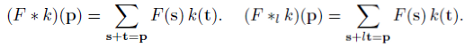
\includegraphics{wiki/1_1.png}
\caption{dilated conv}
\end{figure}

As we can see hyper parameter has been added which is \texttt{l} where
corresponds to number of steps per addition in long-run convolution. If
we set \texttt{l=0}, then we have normal convolution. This parameter
\texttt{l} will skip some points in enighborhood.

Here is how it works:

\begin{figure}
\centering

\includegraphics{wiki/1_2.gif}
\caption{dilated conv vis}
\end{figure}

Dilated convolution incorporates larger receptive field regarding same
amount of parameters of windows size, etc regarding normal conv.

\begin{figure}
\centering
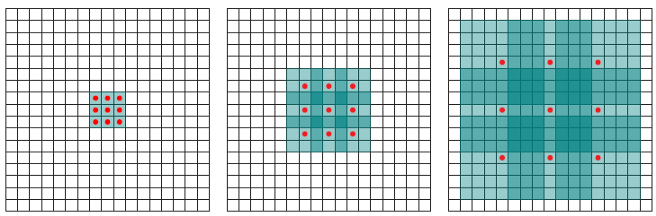
\includegraphics{wiki/1_3.png}
\caption{dilated conv receptive field}
\end{figure}

    \hypertarget{b-use-cases}{%
\subsubsection{1.B Use cases}\label{b-use-cases}}

In the paper
\href{http://vladlen.info/papers/dilated-convolutions.pdf}{Multi-scale
contex aggregation by dilated convolutions} authors have shown that
almost any model on \textbf{semantic segmentation} task can perform
better by adding a \texttt{contex} layer which is constructed of
multiple different conv layers with different size of \texttt{l} to
intorduce bigger receptive field over layers.

The reason is as we know in semantic segmentation of similar tasks, we
need to consider different object sizes when labeling pixels, so by
having normal conv (\texttt{l=1}) and adding dilated convs
(\texttt{l\textgreater{}=2}), the receptive field has been increased so
labeling can be done wiser.

Here is the definition of \texttt{contex} module in the aforementioned
paper:

\begin{figure}
\centering
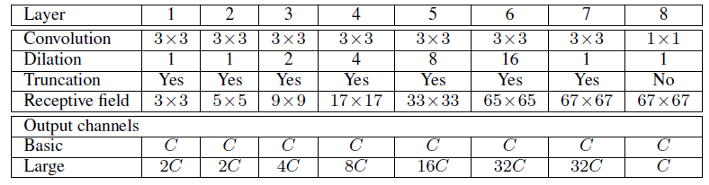
\includegraphics{wiki/1_4.png}
\caption{context module}
\end{figure}

    \hypertarget{c-pros-and-cons}{%
\subsubsection{1.C Pros and Cons}\label{c-pros-and-cons}}

About pros, in summary we can say dilation does not change number of
parameters or calculations, so there is no memory of time disadvantage
about this operation but as this approach provides larger receptive
fields regarding same amount of operations, it outperforms must of the
base models. Also, it dilation factor can be increased while preserving
resolution. All this aspects caused to have better results in semantic
segmentation tasks.

But about cons, using dilation in models such as ResNet where this
models try to preserve learned features in previous layers, can cause
producing artifacts like chess board or dot effect in image-to-image
translation tasks. Although this problem has solved by adding
skip-connections to some particular points, not all x-step convs.

    \hypertarget{mask-r-cnn}{%
\subsection{2 Mask R-CNN:}\label{mask-r-cnn}}

\begin{enumerate}
\def\labelenumi{\arabic{enumi}.}
\tightlist
\item
  Report a summary of
  \href{http://openaccess.thecvf.com/content_ICCV_2017/papers/He_Mask_R-CNN_ICCV_2017_paper.pdf}{Mask
  R-CNN} paper.
\item
  Use any implemented model(pretrained) on your custom input
\end{enumerate}

    \hypertarget{a-mask-r-cnn}{%
\subsubsection{2.A Mask R-CNN}\label{a-mask-r-cnn}}

Let's say firstly we know what is object detection, semantic
segmentation and instance segmentation. (See
\href{https://github.com/Nikronic/Digital-Image-Processing-IUST/tree/master/HW11\#1-compare-semantic-segmentation-object-detection-and-instance-segmentation}{here}
if not)

Also let's say we know what \emph{R-CNN}, \emph{Fast R-CNN} and
\emph{Faster R-CNN} models are. (See
\href{https://github.com/Nikronic/Digital-Image-Processing-IUST/tree/master/HW11\#2-compare-rcnn-fast-rcnn-and-faster-rcnn}{here}
if not)

Mask R-CNN is a model for instance segmentation task. This model
generate 3 outputs : 1. Object label 2. Bounding box 3. Object mask

About all previous models with R-CNN architecture, third output has been
provided and actually the major importance of Mask R-CNN model because
third output.

\emph{Now let's have a brief understanding of model before going into
more details.}

\begin{figure}
\centering
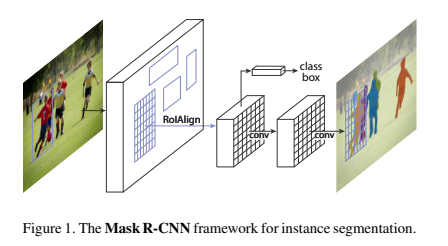
\includegraphics{wiki/2_3.png}
\caption{mask r-cnn model}
\end{figure}

Mask R-CNN has been constructed by two stages, first stage's duty is to
generate region proposals but using completely different approach from
previously proposed papers. Secondly, it generates object labels, refine
boudning boxes and masks pixel-wise based on the region proposal from
first stage. These both stages obtained from a base CNN model based on
\href{https://arxiv.org/abs/1612.03144}{Feature Pyramid Network} style.

FPN is U-net structure where in contracting phase any model like
ResNet101 can be used. There is a expansion phase too which is similar
to contracting phase but reverse in size where the output of each step
in contracting phase has been concatenated to the output of
corresponding layer in expansion phase. Here is image from FPN paper:

\begin{figure}
\centering
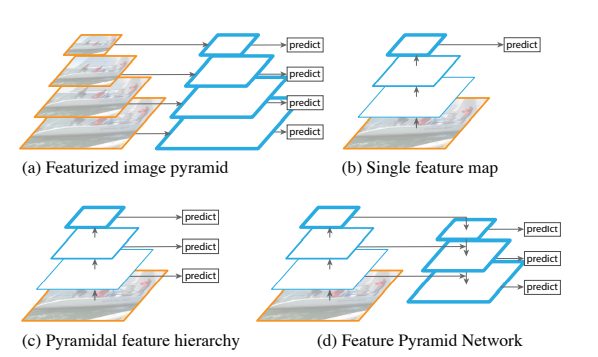
\includegraphics{wiki/2_1.png}
\caption{fpn module}
\end{figure}

\begin{figure}
\centering
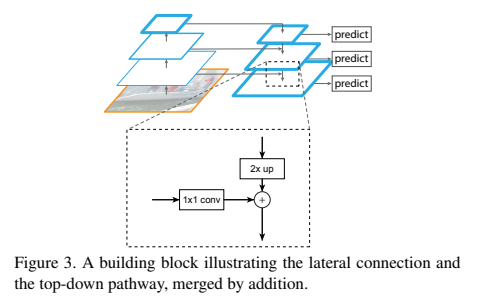
\includegraphics{wiki/2_2.png}
\caption{fpn module concat op}
\end{figure}

Now let's talk about first stage. A small CNN model called RPN (region
proposal network) will extract region candidate where objects may
exists. This model uses the output of expansion phase of FPN model as
input as these inputs are extracted features from input images given to
the whole network. (This step is indentical to Faster R-CNN model)

But for second stage, Mask R-CNN generates a binary mask for each RoI
while predicting object lables and their bounding boxes still is
identical to faster r-cnn and have been done simultaneously.

The loss function also has been expanded to consider mask loss using
weighted sum (for each RoI):

\begin{figure}
\centering
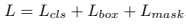
\includegraphics{wiki/2_4.png}
\caption{loss mask rcnn}
\end{figure}

Where loss bounding box and label are identical to faster rcnn.

The mask branch of network has \texttt{Km\^{}2} output where consists of
\texttt{K} layer with size of \texttt{m*m} where \texttt{K} is number of
classes. So loss mask defines in the way that first apply per-pixel
sigmoid then average binary cross-entropy.

Mask representation are small vectors which have been obtained from
fully connected layers. The structure of spatial features of masks can
be gained by pixel-to-pixel measurements. So to do this, authors
generate \texttt{m*m} masks for each RoI using an FCN. But features from
different RoIs need to be well aligned to be correctly measured using
pixel-to-pixel approach and that's why \textbf{RoIAlign} has been
introduced.

\textbf{RoIAlgin} is operation to extract a small feature map from a
RoI. But how it works: 1. Use RoIPool to quantize a floating-point RoI
into discrete form (\texttt{round(x/16)}) 2. Divine output into
different spatial bins where all are quantized too 3. Aggregate feature
values covered by each bin using MaxPool

This approach introduces misaligned bins for different RoIs so to handle
this harsh quantization, \textbf{RoIAlgin} layer has been used. To solve
this issue here is the new approach:

\begin{enumerate}
\def\labelenumi{\arabic{enumi}.}
\tightlist
\item
  Use \texttt{x/16} (no rounding) to quantize
\item
  Consider four bins for each RoI
\item
  Fill missed values using bilinear interpolation
\item
  Aggregate feature values using MaxPool or AvgPool
\end{enumerate}

And about network architecture, three term can represent it: 1.
\textbf{Backbone} where can be any FPN network or VGG style used for
feature extraction 2. \textbf{Head} network for bounding box prediction
and mask generationg where applied \emph{separately} where can be any
fully convolutional network like a part of ResNet, etc.

    \hypertarget{b-mask-r-cnn-inference}{%
\subsubsection{2.B Mask R-CNN Inference}\label{b-mask-r-cnn-inference}}

    \begin{Verbatim}[commandchars=\\\{\}]
{\color{incolor}In [{\color{incolor}5}]:} \PY{o}{!}git clone https://github.com/matterport/Mask\PYZus{}RCNN.git
        \PY{n}{cd} \PY{n}{Mask\PYZus{}RCNN}\PY{o}{/}
\end{Verbatim}


    \begin{Verbatim}[commandchars=\\\{\}]
/content/Mask\_RCNN

    \end{Verbatim}

    \begin{Verbatim}[commandchars=\\\{\}]
{\color{incolor}In [{\color{incolor} }]:} \PY{k+kn}{import} \PY{n+nn}{os}
        \PY{k+kn}{import} \PY{n+nn}{sys}
        \PY{k+kn}{import} \PY{n+nn}{random}
        \PY{k+kn}{import} \PY{n+nn}{math}
        \PY{k+kn}{import} \PY{n+nn}{numpy} \PY{k}{as} \PY{n+nn}{np}
        \PY{k+kn}{import} \PY{n+nn}{skimage}\PY{n+nn}{.}\PY{n+nn}{io}
        \PY{k+kn}{import} \PY{n+nn}{matplotlib}
        \PY{k+kn}{import} \PY{n+nn}{matplotlib}\PY{n+nn}{.}\PY{n+nn}{pyplot} \PY{k}{as} \PY{n+nn}{plt}
        
        \PY{o}{\PYZpc{}}\PY{k}{matplotlib} inline 
        \PY{o}{\PYZpc{}}\PY{k}{tensorflow\PYZus{}version} 1.x
\end{Verbatim}


    \begin{Verbatim}[commandchars=\\\{\}]
{\color{incolor}In [{\color{incolor} }]:} \PY{k+kn}{from} \PY{n+nn}{mrcnn} \PY{k}{import} \PY{n}{utils}
        \PY{k+kn}{import} \PY{n+nn}{mrcnn}\PY{n+nn}{.}\PY{n+nn}{model} \PY{k}{as} \PY{n+nn}{modellib}
        \PY{k+kn}{from} \PY{n+nn}{mrcnn} \PY{k}{import} \PY{n}{visualize}
        \PY{k+kn}{from} \PY{n+nn}{samples}\PY{n+nn}{.}\PY{n+nn}{coco} \PY{k}{import} \PY{n}{coco}
\end{Verbatim}


    \begin{Verbatim}[commandchars=\\\{\}]
{\color{incolor}In [{\color{incolor} }]:} \PY{n}{MODEL\PYZus{}DIR} \PY{o}{=} \PY{l+s+s1}{\PYZsq{}}\PY{l+s+s1}{mask\PYZus{}rcnn\PYZus{}coco.h5}\PY{l+s+s1}{\PYZsq{}}
        \PY{k}{if} \PY{o+ow}{not} \PY{n}{os}\PY{o}{.}\PY{n}{path}\PY{o}{.}\PY{n}{exists}\PY{p}{(}\PY{n}{MODEL\PYZus{}DIR}\PY{p}{)}\PY{p}{:}
            \PY{n}{utils}\PY{o}{.}\PY{n}{download\PYZus{}trained\PYZus{}weights}\PY{p}{(}\PY{n}{MODEL\PYZus{}DIR}\PY{p}{)}
\end{Verbatim}


    \begin{Verbatim}[commandchars=\\\{\}]
{\color{incolor}In [{\color{incolor}16}]:} \PY{k}{class} \PY{n+nc}{InferenceConfig}\PY{p}{(}\PY{n}{coco}\PY{o}{.}\PY{n}{CocoConfig}\PY{p}{)}\PY{p}{:}
             \PY{n}{GPU\PYZus{}COUNT} \PY{o}{=} \PY{l+m+mi}{1}
             \PY{n}{IMAGES\PYZus{}PER\PYZus{}GPU} \PY{o}{=} \PY{l+m+mi}{1}
         
         \PY{n}{config} \PY{o}{=} \PY{n}{InferenceConfig}\PY{p}{(}\PY{p}{)}
         \PY{n}{config}\PY{o}{.}\PY{n}{display}\PY{p}{(}\PY{p}{)}
\end{Verbatim}


    \begin{Verbatim}[commandchars=\\\{\}]

Configurations:
BACKBONE                       resnet101
BACKBONE\_STRIDES               [4, 8, 16, 32, 64]
BATCH\_SIZE                     1
BBOX\_STD\_DEV                   [0.1 0.1 0.2 0.2]
COMPUTE\_BACKBONE\_SHAPE         None
DETECTION\_MAX\_INSTANCES        100
DETECTION\_MIN\_CONFIDENCE       0.7
DETECTION\_NMS\_THRESHOLD        0.3
FPN\_CLASSIF\_FC\_LAYERS\_SIZE     1024
GPU\_COUNT                      1
GRADIENT\_CLIP\_NORM             5.0
IMAGES\_PER\_GPU                 1
IMAGE\_CHANNEL\_COUNT            3
IMAGE\_MAX\_DIM                  1024
IMAGE\_META\_SIZE                93
IMAGE\_MIN\_DIM                  800
IMAGE\_MIN\_SCALE                0
IMAGE\_RESIZE\_MODE              square
IMAGE\_SHAPE                    [1024 1024    3]
LEARNING\_MOMENTUM              0.9
LEARNING\_RATE                  0.001
LOSS\_WEIGHTS                   \{'rpn\_class\_loss': 1.0, 'rpn\_bbox\_loss': 1.0, 'mrcnn\_class\_loss': 1.0, 'mrcnn\_bbox\_loss': 1.0, 'mrcnn\_mask\_loss': 1.0\}
MASK\_POOL\_SIZE                 14
MASK\_SHAPE                     [28, 28]
MAX\_GT\_INSTANCES               100
MEAN\_PIXEL                     [123.7 116.8 103.9]
MINI\_MASK\_SHAPE                (56, 56)
NAME                           coco
NUM\_CLASSES                    81
POOL\_SIZE                      7
POST\_NMS\_ROIS\_INFERENCE        1000
POST\_NMS\_ROIS\_TRAINING         2000
PRE\_NMS\_LIMIT                  6000
ROI\_POSITIVE\_RATIO             0.33
RPN\_ANCHOR\_RATIOS              [0.5, 1, 2]
RPN\_ANCHOR\_SCALES              (32, 64, 128, 256, 512)
RPN\_ANCHOR\_STRIDE              1
RPN\_BBOX\_STD\_DEV               [0.1 0.1 0.2 0.2]
RPN\_NMS\_THRESHOLD              0.7
RPN\_TRAIN\_ANCHORS\_PER\_IMAGE    256
STEPS\_PER\_EPOCH                1000
TOP\_DOWN\_PYRAMID\_SIZE          256
TRAIN\_BN                       False
TRAIN\_ROIS\_PER\_IMAGE           200
USE\_MINI\_MASK                  True
USE\_RPN\_ROIS                   True
VALIDATION\_STEPS               50
WEIGHT\_DECAY                   0.0001



    \end{Verbatim}

    \begin{Verbatim}[commandchars=\\\{\}]
{\color{incolor}In [{\color{incolor} }]:} \PY{n}{model} \PY{o}{=} \PY{n}{modellib}\PY{o}{.}\PY{n}{MaskRCNN}\PY{p}{(}\PY{n}{mode}\PY{o}{=}\PY{l+s+s2}{\PYZdq{}}\PY{l+s+s2}{inference}\PY{l+s+s2}{\PYZdq{}}\PY{p}{,} \PY{n}{model\PYZus{}dir}\PY{o}{=}\PY{l+s+s1}{\PYZsq{}}\PY{l+s+s1}{logs}\PY{l+s+s1}{\PYZsq{}}\PY{p}{,} \PY{n}{config}\PY{o}{=}\PY{n}{config}\PY{p}{)}
        \PY{n}{model}\PY{o}{.}\PY{n}{load\PYZus{}weights}\PY{p}{(}\PY{n}{MODEL\PYZus{}DIR}\PY{p}{,} \PY{n}{by\PYZus{}name}\PY{o}{=}\PY{k+kc}{True}\PY{p}{)}
\end{Verbatim}


    \begin{Verbatim}[commandchars=\\\{\}]
{\color{incolor}In [{\color{incolor}21}]:} \PY{n}{file\PYZus{}name} \PY{o}{=} \PY{l+s+s1}{\PYZsq{}}\PY{l+s+s1}{../conf.jpg}\PY{l+s+s1}{\PYZsq{}}
         \PY{n}{image} \PY{o}{=} \PY{n}{skimage}\PY{o}{.}\PY{n}{io}\PY{o}{.}\PY{n}{imread}\PY{p}{(}\PY{n}{file\PYZus{}name}\PY{p}{)}
         \PY{n}{plt}\PY{o}{.}\PY{n}{imshow}\PY{p}{(}\PY{n}{image}\PY{p}{)}
\end{Verbatim}


\begin{Verbatim}[commandchars=\\\{\}]
{\color{outcolor}Out[{\color{outcolor}21}]:} <matplotlib.image.AxesImage at 0x7feb923cc198>
\end{Verbatim}
            
    \begin{center}
    \adjustimage{max size={0.9\linewidth}{0.9\paperheight}}{output_14_1.png}
    \end{center}
    { \hspace*{\fill} \\}
    
    \begin{Verbatim}[commandchars=\\\{\}]
{\color{incolor}In [{\color{incolor}22}]:} \PY{n}{class\PYZus{}names} \PY{o}{=} \PY{p}{[}\PY{l+s+s1}{\PYZsq{}}\PY{l+s+s1}{BG}\PY{l+s+s1}{\PYZsq{}}\PY{p}{,} \PY{l+s+s1}{\PYZsq{}}\PY{l+s+s1}{person}\PY{l+s+s1}{\PYZsq{}}\PY{p}{,} \PY{l+s+s1}{\PYZsq{}}\PY{l+s+s1}{bicycle}\PY{l+s+s1}{\PYZsq{}}\PY{p}{,} \PY{l+s+s1}{\PYZsq{}}\PY{l+s+s1}{car}\PY{l+s+s1}{\PYZsq{}}\PY{p}{,} \PY{l+s+s1}{\PYZsq{}}\PY{l+s+s1}{motorcycle}\PY{l+s+s1}{\PYZsq{}}\PY{p}{,} \PY{l+s+s1}{\PYZsq{}}\PY{l+s+s1}{airplane}\PY{l+s+s1}{\PYZsq{}}\PY{p}{,}
                        \PY{l+s+s1}{\PYZsq{}}\PY{l+s+s1}{bus}\PY{l+s+s1}{\PYZsq{}}\PY{p}{,} \PY{l+s+s1}{\PYZsq{}}\PY{l+s+s1}{train}\PY{l+s+s1}{\PYZsq{}}\PY{p}{,} \PY{l+s+s1}{\PYZsq{}}\PY{l+s+s1}{truck}\PY{l+s+s1}{\PYZsq{}}\PY{p}{,} \PY{l+s+s1}{\PYZsq{}}\PY{l+s+s1}{boat}\PY{l+s+s1}{\PYZsq{}}\PY{p}{,} \PY{l+s+s1}{\PYZsq{}}\PY{l+s+s1}{traffic light}\PY{l+s+s1}{\PYZsq{}}\PY{p}{,}
                        \PY{l+s+s1}{\PYZsq{}}\PY{l+s+s1}{fire hydrant}\PY{l+s+s1}{\PYZsq{}}\PY{p}{,} \PY{l+s+s1}{\PYZsq{}}\PY{l+s+s1}{stop sign}\PY{l+s+s1}{\PYZsq{}}\PY{p}{,} \PY{l+s+s1}{\PYZsq{}}\PY{l+s+s1}{parking meter}\PY{l+s+s1}{\PYZsq{}}\PY{p}{,} \PY{l+s+s1}{\PYZsq{}}\PY{l+s+s1}{bench}\PY{l+s+s1}{\PYZsq{}}\PY{p}{,} \PY{l+s+s1}{\PYZsq{}}\PY{l+s+s1}{bird}\PY{l+s+s1}{\PYZsq{}}\PY{p}{,}
                        \PY{l+s+s1}{\PYZsq{}}\PY{l+s+s1}{cat}\PY{l+s+s1}{\PYZsq{}}\PY{p}{,} \PY{l+s+s1}{\PYZsq{}}\PY{l+s+s1}{dog}\PY{l+s+s1}{\PYZsq{}}\PY{p}{,} \PY{l+s+s1}{\PYZsq{}}\PY{l+s+s1}{horse}\PY{l+s+s1}{\PYZsq{}}\PY{p}{,} \PY{l+s+s1}{\PYZsq{}}\PY{l+s+s1}{sheep}\PY{l+s+s1}{\PYZsq{}}\PY{p}{,} \PY{l+s+s1}{\PYZsq{}}\PY{l+s+s1}{cow}\PY{l+s+s1}{\PYZsq{}}\PY{p}{,} \PY{l+s+s1}{\PYZsq{}}\PY{l+s+s1}{elephant}\PY{l+s+s1}{\PYZsq{}}\PY{p}{,} \PY{l+s+s1}{\PYZsq{}}\PY{l+s+s1}{bear}\PY{l+s+s1}{\PYZsq{}}\PY{p}{,}
                        \PY{l+s+s1}{\PYZsq{}}\PY{l+s+s1}{zebra}\PY{l+s+s1}{\PYZsq{}}\PY{p}{,} \PY{l+s+s1}{\PYZsq{}}\PY{l+s+s1}{giraffe}\PY{l+s+s1}{\PYZsq{}}\PY{p}{,} \PY{l+s+s1}{\PYZsq{}}\PY{l+s+s1}{backpack}\PY{l+s+s1}{\PYZsq{}}\PY{p}{,} \PY{l+s+s1}{\PYZsq{}}\PY{l+s+s1}{umbrella}\PY{l+s+s1}{\PYZsq{}}\PY{p}{,} \PY{l+s+s1}{\PYZsq{}}\PY{l+s+s1}{handbag}\PY{l+s+s1}{\PYZsq{}}\PY{p}{,} \PY{l+s+s1}{\PYZsq{}}\PY{l+s+s1}{tie}\PY{l+s+s1}{\PYZsq{}}\PY{p}{,}
                        \PY{l+s+s1}{\PYZsq{}}\PY{l+s+s1}{suitcase}\PY{l+s+s1}{\PYZsq{}}\PY{p}{,} \PY{l+s+s1}{\PYZsq{}}\PY{l+s+s1}{frisbee}\PY{l+s+s1}{\PYZsq{}}\PY{p}{,} \PY{l+s+s1}{\PYZsq{}}\PY{l+s+s1}{skis}\PY{l+s+s1}{\PYZsq{}}\PY{p}{,} \PY{l+s+s1}{\PYZsq{}}\PY{l+s+s1}{snowboard}\PY{l+s+s1}{\PYZsq{}}\PY{p}{,} \PY{l+s+s1}{\PYZsq{}}\PY{l+s+s1}{sports ball}\PY{l+s+s1}{\PYZsq{}}\PY{p}{,}
                        \PY{l+s+s1}{\PYZsq{}}\PY{l+s+s1}{kite}\PY{l+s+s1}{\PYZsq{}}\PY{p}{,} \PY{l+s+s1}{\PYZsq{}}\PY{l+s+s1}{baseball bat}\PY{l+s+s1}{\PYZsq{}}\PY{p}{,} \PY{l+s+s1}{\PYZsq{}}\PY{l+s+s1}{baseball glove}\PY{l+s+s1}{\PYZsq{}}\PY{p}{,} \PY{l+s+s1}{\PYZsq{}}\PY{l+s+s1}{skateboard}\PY{l+s+s1}{\PYZsq{}}\PY{p}{,}
                        \PY{l+s+s1}{\PYZsq{}}\PY{l+s+s1}{surfboard}\PY{l+s+s1}{\PYZsq{}}\PY{p}{,} \PY{l+s+s1}{\PYZsq{}}\PY{l+s+s1}{tennis racket}\PY{l+s+s1}{\PYZsq{}}\PY{p}{,} \PY{l+s+s1}{\PYZsq{}}\PY{l+s+s1}{bottle}\PY{l+s+s1}{\PYZsq{}}\PY{p}{,} \PY{l+s+s1}{\PYZsq{}}\PY{l+s+s1}{wine glass}\PY{l+s+s1}{\PYZsq{}}\PY{p}{,} \PY{l+s+s1}{\PYZsq{}}\PY{l+s+s1}{cup}\PY{l+s+s1}{\PYZsq{}}\PY{p}{,}
                        \PY{l+s+s1}{\PYZsq{}}\PY{l+s+s1}{fork}\PY{l+s+s1}{\PYZsq{}}\PY{p}{,} \PY{l+s+s1}{\PYZsq{}}\PY{l+s+s1}{knife}\PY{l+s+s1}{\PYZsq{}}\PY{p}{,} \PY{l+s+s1}{\PYZsq{}}\PY{l+s+s1}{spoon}\PY{l+s+s1}{\PYZsq{}}\PY{p}{,} \PY{l+s+s1}{\PYZsq{}}\PY{l+s+s1}{bowl}\PY{l+s+s1}{\PYZsq{}}\PY{p}{,} \PY{l+s+s1}{\PYZsq{}}\PY{l+s+s1}{banana}\PY{l+s+s1}{\PYZsq{}}\PY{p}{,} \PY{l+s+s1}{\PYZsq{}}\PY{l+s+s1}{apple}\PY{l+s+s1}{\PYZsq{}}\PY{p}{,}
                        \PY{l+s+s1}{\PYZsq{}}\PY{l+s+s1}{sandwich}\PY{l+s+s1}{\PYZsq{}}\PY{p}{,} \PY{l+s+s1}{\PYZsq{}}\PY{l+s+s1}{orange}\PY{l+s+s1}{\PYZsq{}}\PY{p}{,} \PY{l+s+s1}{\PYZsq{}}\PY{l+s+s1}{broccoli}\PY{l+s+s1}{\PYZsq{}}\PY{p}{,} \PY{l+s+s1}{\PYZsq{}}\PY{l+s+s1}{carrot}\PY{l+s+s1}{\PYZsq{}}\PY{p}{,} \PY{l+s+s1}{\PYZsq{}}\PY{l+s+s1}{hot dog}\PY{l+s+s1}{\PYZsq{}}\PY{p}{,} \PY{l+s+s1}{\PYZsq{}}\PY{l+s+s1}{pizza}\PY{l+s+s1}{\PYZsq{}}\PY{p}{,}
                        \PY{l+s+s1}{\PYZsq{}}\PY{l+s+s1}{donut}\PY{l+s+s1}{\PYZsq{}}\PY{p}{,} \PY{l+s+s1}{\PYZsq{}}\PY{l+s+s1}{cake}\PY{l+s+s1}{\PYZsq{}}\PY{p}{,} \PY{l+s+s1}{\PYZsq{}}\PY{l+s+s1}{chair}\PY{l+s+s1}{\PYZsq{}}\PY{p}{,} \PY{l+s+s1}{\PYZsq{}}\PY{l+s+s1}{couch}\PY{l+s+s1}{\PYZsq{}}\PY{p}{,} \PY{l+s+s1}{\PYZsq{}}\PY{l+s+s1}{potted plant}\PY{l+s+s1}{\PYZsq{}}\PY{p}{,} \PY{l+s+s1}{\PYZsq{}}\PY{l+s+s1}{bed}\PY{l+s+s1}{\PYZsq{}}\PY{p}{,}
                        \PY{l+s+s1}{\PYZsq{}}\PY{l+s+s1}{dining table}\PY{l+s+s1}{\PYZsq{}}\PY{p}{,} \PY{l+s+s1}{\PYZsq{}}\PY{l+s+s1}{toilet}\PY{l+s+s1}{\PYZsq{}}\PY{p}{,} \PY{l+s+s1}{\PYZsq{}}\PY{l+s+s1}{tv}\PY{l+s+s1}{\PYZsq{}}\PY{p}{,} \PY{l+s+s1}{\PYZsq{}}\PY{l+s+s1}{laptop}\PY{l+s+s1}{\PYZsq{}}\PY{p}{,} \PY{l+s+s1}{\PYZsq{}}\PY{l+s+s1}{mouse}\PY{l+s+s1}{\PYZsq{}}\PY{p}{,} \PY{l+s+s1}{\PYZsq{}}\PY{l+s+s1}{remote}\PY{l+s+s1}{\PYZsq{}}\PY{p}{,}
                        \PY{l+s+s1}{\PYZsq{}}\PY{l+s+s1}{keyboard}\PY{l+s+s1}{\PYZsq{}}\PY{p}{,} \PY{l+s+s1}{\PYZsq{}}\PY{l+s+s1}{cell phone}\PY{l+s+s1}{\PYZsq{}}\PY{p}{,} \PY{l+s+s1}{\PYZsq{}}\PY{l+s+s1}{microwave}\PY{l+s+s1}{\PYZsq{}}\PY{p}{,} \PY{l+s+s1}{\PYZsq{}}\PY{l+s+s1}{oven}\PY{l+s+s1}{\PYZsq{}}\PY{p}{,} \PY{l+s+s1}{\PYZsq{}}\PY{l+s+s1}{toaster}\PY{l+s+s1}{\PYZsq{}}\PY{p}{,}
                        \PY{l+s+s1}{\PYZsq{}}\PY{l+s+s1}{sink}\PY{l+s+s1}{\PYZsq{}}\PY{p}{,} \PY{l+s+s1}{\PYZsq{}}\PY{l+s+s1}{refrigerator}\PY{l+s+s1}{\PYZsq{}}\PY{p}{,} \PY{l+s+s1}{\PYZsq{}}\PY{l+s+s1}{book}\PY{l+s+s1}{\PYZsq{}}\PY{p}{,} \PY{l+s+s1}{\PYZsq{}}\PY{l+s+s1}{clock}\PY{l+s+s1}{\PYZsq{}}\PY{p}{,} \PY{l+s+s1}{\PYZsq{}}\PY{l+s+s1}{vase}\PY{l+s+s1}{\PYZsq{}}\PY{p}{,} \PY{l+s+s1}{\PYZsq{}}\PY{l+s+s1}{scissors}\PY{l+s+s1}{\PYZsq{}}\PY{p}{,}
                        \PY{l+s+s1}{\PYZsq{}}\PY{l+s+s1}{teddy bear}\PY{l+s+s1}{\PYZsq{}}\PY{p}{,} \PY{l+s+s1}{\PYZsq{}}\PY{l+s+s1}{hair drier}\PY{l+s+s1}{\PYZsq{}}\PY{p}{,} \PY{l+s+s1}{\PYZsq{}}\PY{l+s+s1}{toothbrush}\PY{l+s+s1}{\PYZsq{}}\PY{p}{]}
         
         \PY{c+c1}{\PYZsh{} Run detection}
         \PY{n}{results} \PY{o}{=} \PY{n}{model}\PY{o}{.}\PY{n}{detect}\PY{p}{(}\PY{p}{[}\PY{n}{image}\PY{p}{]}\PY{p}{,} \PY{n}{verbose}\PY{o}{=}\PY{l+m+mi}{1}\PY{p}{)}
         
         \PY{c+c1}{\PYZsh{} Visualize results}
         \PY{n}{r} \PY{o}{=} \PY{n}{results}\PY{p}{[}\PY{l+m+mi}{0}\PY{p}{]}
         \PY{n}{visualize}\PY{o}{.}\PY{n}{display\PYZus{}instances}\PY{p}{(}\PY{n}{image}\PY{p}{,} \PY{n}{r}\PY{p}{[}\PY{l+s+s1}{\PYZsq{}}\PY{l+s+s1}{rois}\PY{l+s+s1}{\PYZsq{}}\PY{p}{]}\PY{p}{,} \PY{n}{r}\PY{p}{[}\PY{l+s+s1}{\PYZsq{}}\PY{l+s+s1}{masks}\PY{l+s+s1}{\PYZsq{}}\PY{p}{]}\PY{p}{,} \PY{n}{r}\PY{p}{[}\PY{l+s+s1}{\PYZsq{}}\PY{l+s+s1}{class\PYZus{}ids}\PY{l+s+s1}{\PYZsq{}}\PY{p}{]}\PY{p}{,} \PY{n}{class\PYZus{}names}\PY{p}{,} \PY{n}{r}\PY{p}{[}\PY{l+s+s1}{\PYZsq{}}\PY{l+s+s1}{scores}\PY{l+s+s1}{\PYZsq{}}\PY{p}{]}\PY{p}{)}
\end{Verbatim}


    \begin{Verbatim}[commandchars=\\\{\}]
Processing 1 images
image                    shape: (852, 1280, 3)        min:    0.00000  max:  255.00000  uint8
molded\_images            shape: (1, 1024, 1024, 3)    min: -123.70000  max:  151.10000  float64
image\_metas              shape: (1, 93)               min:    0.00000  max: 1280.00000  float64
anchors                  shape: (1, 261888, 4)        min:   -0.35390  max:    1.29134  float32

    \end{Verbatim}

    \begin{center}
    \adjustimage{max size={0.9\linewidth}{0.9\paperheight}}{output_15_1.png}
    \end{center}
    { \hspace*{\fill} \\}
    
    \emph{Note: README: The code has been run on Colab}

    \hypertarget{compute-number-of-parameters-in-each-layer-for-below-network}{%
\subsection{\texorpdfstring{3 Compute number of parameters \emph{in each
layer} for below
network:}{3 Compute number of parameters in each layer for below network:}}\label{compute-number-of-parameters-in-each-layer-for-below-network}}

``` python model = get\_unet((256, 256, 3)) def
conv2d\_block(input\_tensor, n\_filters, kernel\_size=3):

\# first layer x=Conv2D(filters=n\_filters, kernel\_size=(kernel\_size,
kernel\_size), padding=`same')(input\_tensor) \# Block\_\{changes with
`c' layers\}\emph{1 x=Activation(`relu')(x) \# second layer
x=Conv2D(filters=n\_filters, kernel\_size=(kernel\_size, kernel\_size),
padding=`same')(input\_tensor) \# Block}\{changes with `c' layers\}\_2
x=Activation(`relu')(x) return x def get\_unet(input\_img,
n\_filters=16): \# Contracting Path c1=conv2d\_block(input\_img,
n\_filters*1, kernel\_size=3) \# c1 p1=MaxPooling2D((2, 2))(c1)

c2=conv2d\_block(p1, n\_filters*2, kernel\_size=3) \# c2
p2=MaxPooling2D((2, 2))(c2)

c3=conv2d\_block(p2, n\_filters*4, kernel\_size=3) \# c3
p3=MaxPooling2D((2, 2))(c3)

c4=conv2d\_block(p3, n\_filters*8, kernel\_size=3) \# c4
p4=MaxPooling2D((2, 2))(c4)

c5=conv2d\_block(p4, n\_filters=n\_filters*16, kernel\_size=3) \# c5

\# Expansive Path u6=Conv2DTranspose(n\_filters\emph{8, (3, 3),
strides=(2, 2), padding=`same')(c5) \# u6 u6=concatenate({[}u6, c4{]})
c6=conv2d\_block(u6, n\_filters}8, kernel\_size=3) \# c6
u7=Conv2DTranspose(n\_filters*4, (3, 3), strides=(2, 2),
padding=`same')(c6) \# u7 u7=concatenate({[}u7, c3{]})

c7=conv2d\_block(u7, n\_filters\emph{4, kernel\_size=3) \# c7
u8=Conv2DTranspose(n\_filters}2, (3, 3), strides=(2, 2),
padding=`same')(c7) \# u8 u8=concatenate({[}u8, c2{]})
c8=conv2d\_block(u8, n\_filters\emph{2, kernel\_size=3) \# c8
u9=Conv2DTranspose(n\_filters}1, (3, 3), strides=(2, 2),
padding=`same')(c8) \# u9 u9=concatenate({[}u9, c1{]})
c9=conv2d\_block(u9, n\_filters*1, kernel\_size=3) \#c9
outputs=Conv2D(10, (1, 1), activation=`sigmoid')(c9) \# outputs
model=Model(inputs={[}input\_img{]}, outputs={[}outputs{]}) return model

    First please the comments above the understand naming convention used in
below table of number of paramteres demonstration.

\begin{longtable}[]{@{}ll@{}}
\toprule
Layer Name & \# Params\tabularnewline
\midrule
\endhead
block\_c1\_1 & 448\tabularnewline
block\_c1\_2 & 2320\tabularnewline
block\_c2\_1 & 4640\tabularnewline
block\_c2\_2 & 9248\tabularnewline
block\_c3\_1 & 18496\tabularnewline
block\_c3\_2 & 36928\tabularnewline
block\_c4\_1 & 73856\tabularnewline
block\_c4\_2 & 147584\tabularnewline
block\_c5\_1 & 295168\tabularnewline
block\_c5\_2 & 590080\tabularnewline
u6 & 295040\tabularnewline
block\_c6\_1 & 295040\tabularnewline
block\_c6\_2 & 147584\tabularnewline
u7 & 73792\tabularnewline
block\_c7\_1 & 73792\tabularnewline
block\_c7\_2 & 36928\tabularnewline
u8 & 18464\tabularnewline
block\_c8\_1 & 18464\tabularnewline
block\_c8\_2 & 9248\tabularnewline
u9 & 4624\tabularnewline
block\_c9\_1 & 4624\tabularnewline
block\_c9\_2 & 2320\tabularnewline
outputs & 170\tabularnewline
\bottomrule
\end{longtable}


    % Add a bibliography block to the postdoc
    
    
    
    \end{document}
